% Diese Zeile bitte -nicht- aendern.
\documentclass[course=erap]{aspdoc}

\usepackage{graphicx}
\usepackage{amsmath}

%%%%%%%%%%%%%%%%%%%%%%%%%%%%%%%%%
%% TODO: Ersetzen Sie in den folgenden Zeilen die entsprechenden -Texte-
%% mit den richtigen Werten.
\newcommand{\theGroup}{158} % Beispiel: 158
\newcommand{\theNumber}{A206} % Beispiel: A206
\author{Lukas Li \and Yassine Hmidi \and Constantin Carste}
\date{Wintersemester 2023/24} % Beispiel: Wintersemester 2023/24
%%%%%%%%%%%%%%%%%%%%%%%%%%%%%%%%%

% Diese Zeile bitte -nicht- aendern.
\title{Gruppe \theGroup{} -- Abgabe zu Aufgabe \theNumber}

\begin{document}
\maketitle

\section{Einleitung}
Im Bereich der digitalen Bildverarbeitung führt die Schnittstelle zwischen mathematischen Prinzipien und realer Anwendung zu vielen innovativen Algorithmen, die den jetzigen Stand der Technik verbessert. Dieses Projekt befasst sich mit der Bildmanipulation und spezialisiert sich insbesondere auf die Umwandlung von Farbbildern in Graustufen und eine anschließende Skalierung durch bilineare Interpolation. Dazu werden theoretische Erkenntnisse aus der Mathematik genutzt, um einem praktischen C-Algorithmus zu entwickeln.\\\\
Jedes Farbbild besteht aus Pixeln, die durch ihre Position (x, y) eindeutig identifiziert und durch ihren Farbvektor (R, G, B) definiert werden. Die erste Herausforderung besteht darin, diese Farbpixel in Graustufen umzuwandeln. Dabei wird ein gewichteter Durchschnitt der Einträge des Farbvektors mit geeigneten Koeffizienten a, b und c berechnet. Bei der Berechnung der Grauwerte wird Rücksicht auf die Wahrnehmung des menschlichen visuellen Systems (HVS) genommen, damit das entstandene Graustufenbild besonders ansprechend für die menschlichen Augen ist. Anschließend wird die bilineare Interpolation angewendet, um das Bild passend zu skalieren.\\\\
Die theoretische Grundlage dieses Projekts basiert auf dem Verständnis des 24bpp PPM-Bildformats, welches als Eingabe erwartet wird, sowie auf den mathematischen Berechnungen der Graustufenkonvertierung und der bilinearen Interpolation.\\\\
Auf der praktischen Seite erstreckt sich die Aufgabe über die Umsetzung der theoretischen Erkenntnisse in der Programmiersprache C. Die Implementierung des Algorithmus umfasst ebenso ein Rahmenprogramm, das PPM-Dateien und weitere optionale Parameter über die Kommandozeile entgegennimmt und das Ergebnis der Berechnung als ein PGM-Bild abspeichert. Durch die I/O-Funktionen des Rahmenprogramms wird eine praktische Einbindung des Resultats in weitere Projekte und das Anpassen des Algorithmus an verschiedene Szenarien ermöglicht.\\\\
Während der Ausarbeitung des Projektes wird insbesondere der Fokus auf die Optimierung gelegt – theoretisch durch algorithmische Optimierung und praktisch durch Parallelisierung und SIMD. Das besondere Interesse an der Beschleunigung des Codes soll die maximale Performance anbieten, damit die maximale Zufriedenheit für den potenziellen Nutzer des Programmes gewährleistet wird.
\section{Lösungsansatz}
Das Programm muss die Nutzereingaben korrekt erkennen und bei fehlerhaften Eingaben sinnvolle Alternativwerte verwenden.
Die eigentliche Konvertierung wird in drei Teilsektionen aufgeteilt. Die Graustufenkonvertierung konvertiert die PPM-Eingabe zu einem PGM-Bild, die Interpolation skaliert das PGM Bild mit dem vom Benutzer angegebenen Faktor und gibt dieses aus.

\begin{figure}[h]
    \centering
    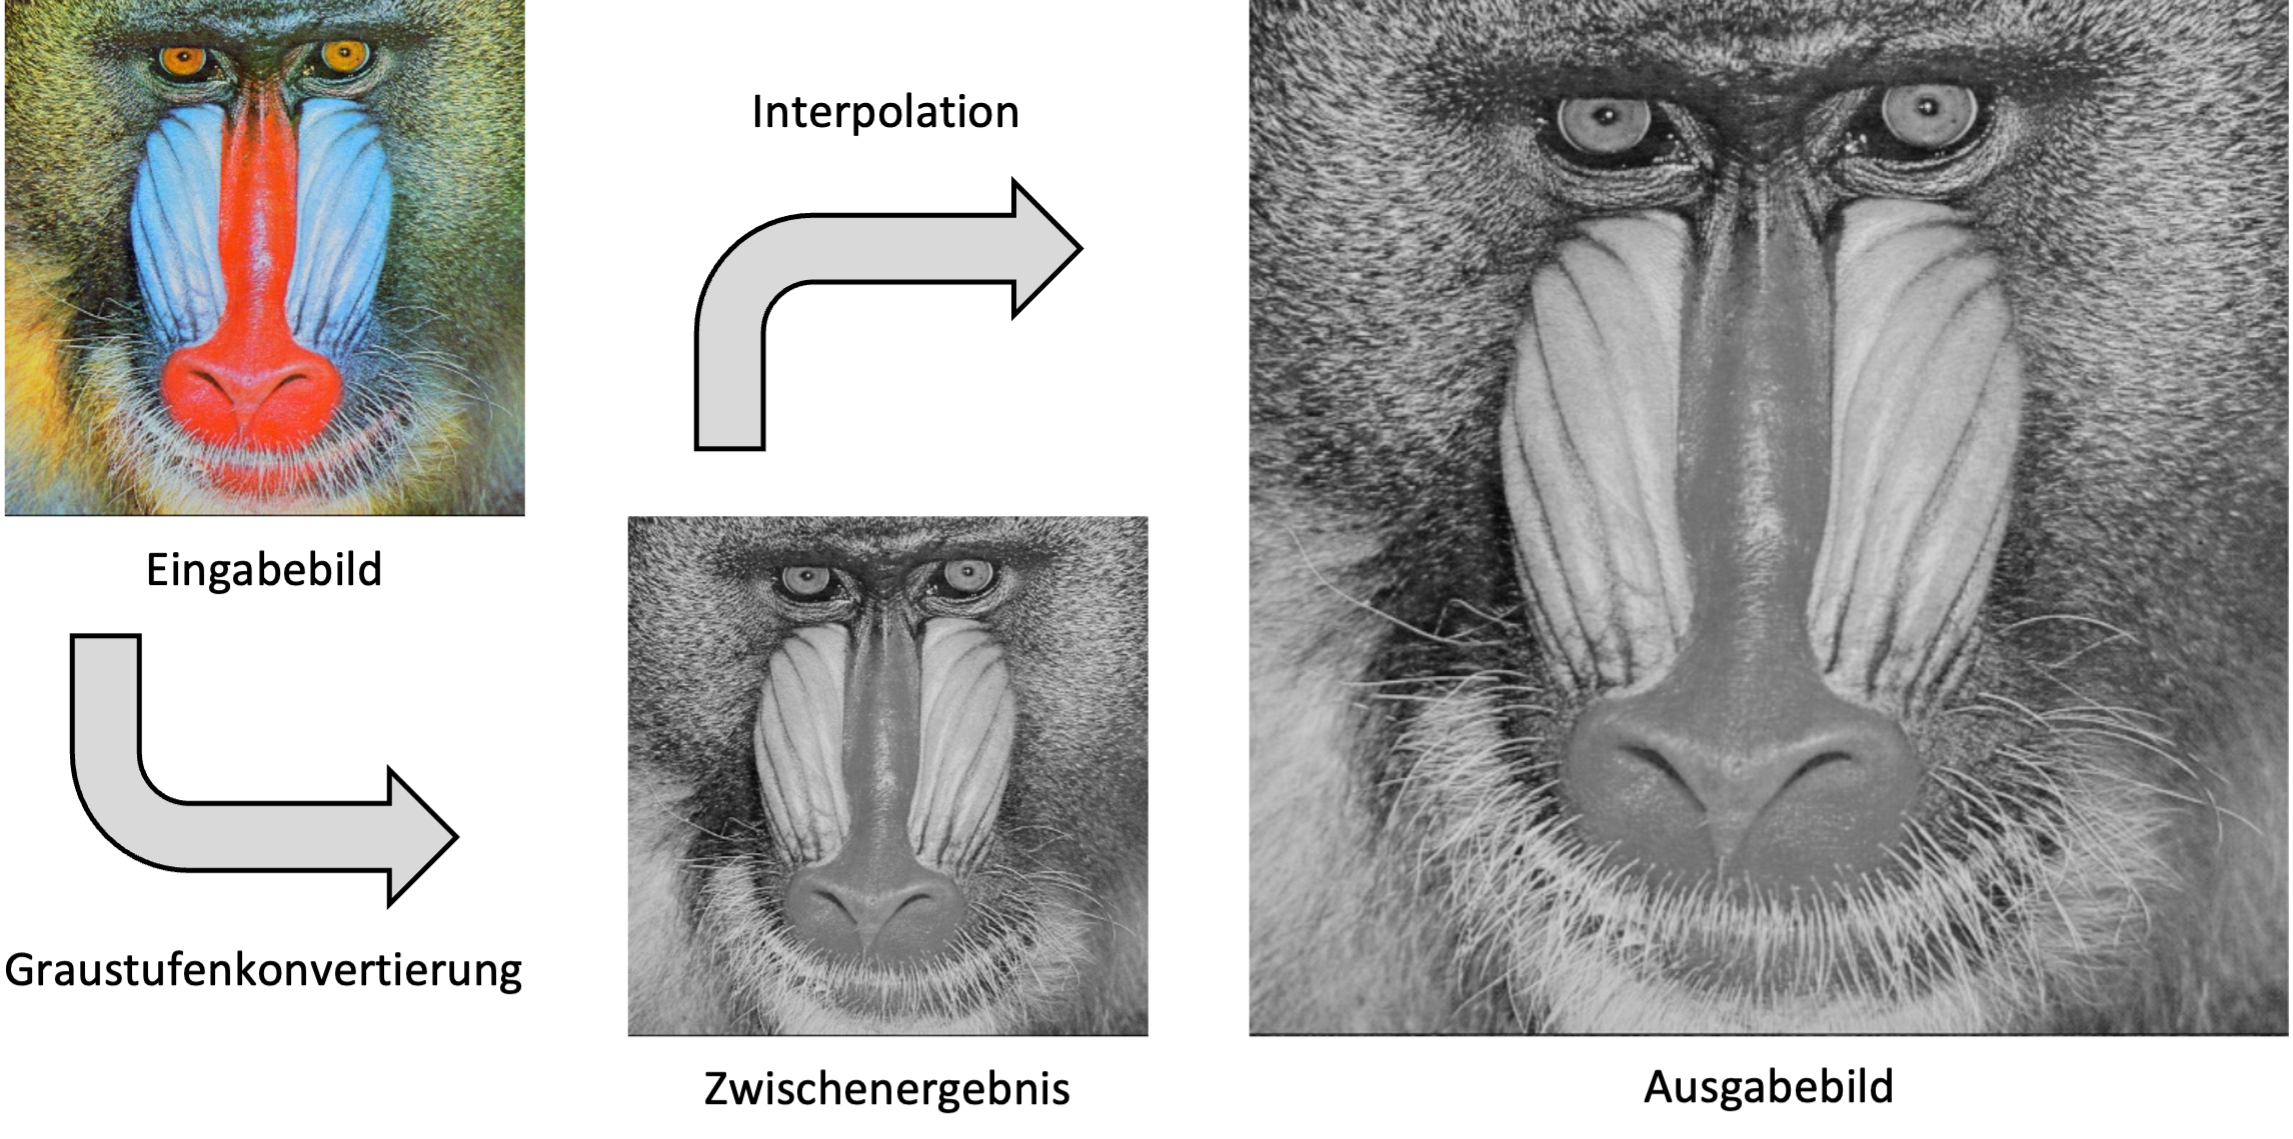
\includegraphics[scale=0.8]{Ausarbeitung/assets/verlauf.png}
    \caption{Verlauf der Eingabe zur fertigen Ausgabe}
    \label{fig:verlauf}
\end{figure}

\subsection{Rahmenprogramm}
Im Zuge der Implementierung war es nötig, einen Rahmenprogramm für angenehme Benutzererfahrung zu erstellen. Dabei wurde besonders viel Rücksicht auf die Benutzerfreundlichkeit genommen. So ist es möglich, die optionalen Parametern ./implementation -V 0 -B 1 -o output.pgm --coeffs a,b,c -f 2 eingabe.ppm zu verwenden. Bis auf das Eingabebild sind alle Parametern optional und müssen nicht gesetzt werden. Dabei wird als Eingabebild ein 24bpp P6 ppm Bild erwartet (das heißt, für jede Farbkanal Rot, Grün und Blau darf nicht mehr als ein Byte verwendet werden, außerdem, darf die Luminanz nicht gesetzt werden). Falls die Parametern nicht gesetzt oder falsch sind wie zum Beispiel ungültige Dateiname für Ausgabedateien, dann wird nach eine kurze Warnung auf der Konsole auf Standardwerte zurückgegriffen. Dabei gibt -V 0 die verwendete Implementation, -B 1 die Anzahl der Wiederholungen beim Benchmark, -o output.pgm die Ausgabedatei, und --coeffs a,bc die zu verwendende Koeffizienten der Graustufenkonvertierung und -f 2 den Skalierungsfaktor beim Interpolieren an. Des Weiteren gibt es noch den Parametern -h / --help, deren Aufruf den Benutzer eine Beschreibung aller Optionen und Benutzerbeispiele anzeigt. Die Standardwerte sind: -V 0 -o output.pgm --coeffs $0.299,0.587,0.114$ und -f 2. Normalerweise wird -B 1 gar nicht gesetzt, da beim gesetzten -B die verwendeten Implementation auf Zeit gemessen wird. Die Koeffizienten $0.299, 0.587$ und $0.144$ sind aufgrund der Annahme, dass das menschliche Auge Grün stärker als Rot und Rot stärker als Blau wahrnimmt, getroffen. Damit ergibt sich ein dem menschlichen Wahrnehmungssystem besonders ansprechende Graustufenbild. Nach dem die Eingaben auf ihre Richtigkeit geprüft beziehungsweise auf Standardwerte gesetzt wurden, wird die Funktion void interpolate(const uint8\_t* img, size\_t width, size\_t height, float a, float b, float c, size\_t scale\_factor, uint8\_t* tmp, uint8\_t* result) aufgerufen. Allerdings wird beim fehlende Parameter für das Eingabebild oder ungültiges Eingabebild wie falsches Bildformat mit einer Fehlermeldung des Problems abgebrochen, da das Programm keinen sinnvollen Standardwert außer einen vorher gespeicherten Bild anbieten könnte, was nicht wirklich sinnvoller ist. Die Funktion interpolate(…) speichert das Graustufenbild in tmp und das interpolierte Bild in result ab. Anschließend schreibt das Rahmenprogramm das Bild als ein P5 pgm-Bild unter den gesetzten Parameter in den Speicher.

\subsection{Graustufenkonvertierung}
Die Graustufenkonvertierung sieht vor, das vom Benuter angegebene PPM Bild in ein PGM-Bild umzuwandeln. Ein PPM-Bild hat für jeden Pixel drei Werte gegeben (R,G,B), ein PGM-Bild nur einen. Die R,G und B Werte müssen also mit Koeffizienten (a,b und c), die vom Benutzer oder Rahmenprogramm gegeben werden, zu einem einzelnen Wert D konvertiert werden.
 \begin{align}
    D_{neu} {=} \frac{a \cdot R + b \cdot B + c \cdot D}{a + b + c}
\end{align}
Um jede Konvertierung zu optimieren muss $a + b + c = 1$ gegeben sein, da dadurch eine Division für jeden Pixel gespart werden kann. Die Koeffizienten werden also vor Konvertierung miteinander skaliert.
 \begin{align}
    D_{neu} \underset{a + b + c = 1}{=} a \cdot R + b \cdot B + c \cdot D
\end{align}


\subsubsection{Naive Konvertierung}
Die naive Konvertierung sieht vor, jeden Pixel einzeln zu berechnen und als neues Bild abzuspeichern. Die Konvertierung wird mit der Rundstrategie durchgeführt, um den Quantisierungsfehler zu minimieren, der durch eine Konvertierung von float zu int entsteht. Dadurch werden die Graustufenintensitäten sichergestellt und die Helligkeitsstufen im ursprünglichen Farbbild garantiert, wodurch das resultierende Bild mehr Details erhält.

\subsubsection{Konvertierung mit Tabellen}
Für diesen Konvertierungsansatz werden vorberechnete Tabellen verwendet, die jedes mögliche Ergebnis der Multiplikation von 0 bis 255 (bzw. dem maximalen Farbwert) mit den entsprechenden Koeffizienten liefern. Aufgrund der Größenlimitierung durch den Farbwert könnte ihre Zuweisung lokal im Stack verfolgen. Die Idee ist, doppelte Berechnungen von Werten zu vermeiden. Die drei Ergebnisse werden daraufhin addiert, um den endgültigen PGM-Pixel zu erhalten.

\subsubsection{Konvertierung mit SIMD}
Die SIMD-Konvertierung verarbeitet jeweils vier Pixel gleichzeitig, um die Leistung gegenüber einer sequenziellen Bearbeitung zu steigern. Zu Beginn werden die Farbkanäle und ein weiterer Vektor initialisiert, der zur letztendlichen Konvertierung zu uint8\_t verwendet wird. Ebenfalls werden drei weitere Vektoren für die Zwischenwerte der Multiplikation vorbereitet. Da SIMD ausgerichtete Daten voraussetzt, durchlaufen wir die letzten Pixel nicht mit SIMD.\\
Jeder Farbkanal wird auf die nächsten R-, G- oder B-Werte gesetzt und mit ihren entsprechenden Vektorkoeffizienten multipliziert und daraufhin auf D aufaddiert. Das fertige PGM-Bild kann daraufhin an die Interpolation weitergegeben werden.

\subsection{Interpolation}
Das Ziel der Interpolation ist es, eine Bildskalierung durchzuführen, also ein Bild so zu vergrößern, dass das menschliche Auge möglichst wenig Unschärfe erkennen kann. Hierfür werden einzelne Pixel mit einem Skalierungsfaktor $k$ voneinander verschoben, wodurch Löcher von $k-1$ Pixeln im neu generierten Bild entstehen, welche mit Zwischenwerten aufgefüllt werden. Zwei zuvor aneinandergrenzende Pixel mit $k = 2$, einer schwarz, der andere weiß, sollte also in einem grauen Pixel resultieren. Da die Verschiebung in der Höhe sowie Breite durchgeführt wird entsteht pro Pixel ein neues Quadrat der Größe $k \cdot k$, mit dem Pixel in der oberen linken Ecke. Durch Ausweitung des Quadrats auf $(k+1) \cdot (k+1)$ erhält man
ein Quadrat, dessen Eckpunkte bekannt sind. Anhand der bekannten Pixel kann man die restlichen Pixel mit der folgenden Formel berechnen und befüllen. Für die mathematische Berechnung werden die Pixel in einem Koordinatensystem mit $x, y \in [0, k+1]$ angegeben. Also haben die vier originalen Eck-Pixel folgende Koordinaten: $(0, 0), (0, k+1), (k+1, 0)$ und $(k+1, k+1)$. Für die unbekannten zu interpolierenden Pixel gilt dann die Formel
 \begin{align}
    Q_{neu} {=}  \frac{1}{(k+1)^2} \cdot
    \begin{pmatrix} k+1-y & y \end{pmatrix} \cdot
    \begin{pmatrix} Q_{(0,0)} & Q_{(0,k+1)} \\ Q_{(k+1,0)} & Q_{(k+1,k+1)} \end{pmatrix}
    \cdot
     \begin{pmatrix} k+1-x \\ x \end{pmatrix} 
\end{align}

 
mit $(x, y)$ als Koordinaten des zu berechnenden Pixels. Diese Funktion funktioniert für fast alle Quadrate, mit Ausnahme der rechten und unteren, da diese keine Nachbar-Pixel haben, auf die das Quadrat ausgeweitet werden kann. Um die Interpolation weiter durchzuführen müssen also sinnvolle Alternativwerte gefunden werden.

\subsection{Interpolation der Randpunkte}
Bei der Interpolation der rechten sowie unteren Randpixel fehlen jeweils zwei bis drei der vier benötigten Eckpunkte (letzteres nur in der unteren rechten Ecke). Für diese Interpolation müssen also Alternativwerte gesucht werden.

\subsubsection{Unbekannte Eckpunkte als Schwarze oder Weiße Pixel annehmen}
Der erste Ansatz, alle unbekannten Werte auf $0$ oder auf den maximalen Farbwert ($255$) zu setzen, würde bei einem überwiegend schwarzen oder weißen Bild zu einem ungewollten Graustufenverlauf führen. (Beispiel: Portrait mit weißem Hintergrund und schwarzen unbekannten Pixeln führt an den Rändern zu einem kleinen Schatten-Effekt)

\subsubsection{Unbekannte Eckpunkte auf die benachbarten bekannten Eckpunkte setzen}
Wenn die Werte des benachbarten Wertes übernommen werden, gleichen alle interpolierten Werte dazwischen ebenfalls diesem Wert. (Beispiel: Eine Interpolation zwischen weiß und weiß ergibt weiß) Das würde an den zwei Kanten zu langgezogenen gleichfarbigen Linien führen, in der unteren rechten Ecke zu einem komplett gleichfarbigen Quadrat. Dieses Problem wird erst bei einem höheren Faktor sichtbar.

\subsubsection{Unbekannte Eckpunkte auf den gegenüberliegend ersten Wert setzen}
Zum Verständnis sehen wir das Bild als Zyliner an. Dadurch berühren sich zwei Kanten, als Beispiel die linke und rechte Kante, lösen also das Problem der unbekannten Eckpunkte für eine Kante auf. Im Klartext füllt man somit die unbekannten Eckpunkte mit den ersten Eckpunkten der aktuell bearbeitenden Reihe / Spalte. Die Implementierung löst die Probleme der anderen Ansätze, würde jedoch bspsweise bei einem Verlaufsbild von schwarz nach weiß zu einer ungewollten rechten Kante führen. Die meisten Bilder, haben jedoch einen gleichfarbigen Farbverlauf von links nach rechts (wie beispielsweise der Horizont eines Portraits), der unwahrscheinliche Fall des Verlaufsbild kann also ausgenommen werden.


\subsection{Naive Interpolationsansätze}

\subsection{Erster Naiver Interpolationsansatz}
Der erste Interpolationsansatz sieht vor, dass für jeden Pixel die Randpunkte $a, b, c, d$ berechnet werden und anhand der Formel der Pixel berechnet und abgespeichert wird. In diesem Ansatz findet fast keine Optimierung statt und ist damit auch der langsamste Ansatz.

\subsection{Zweiter Naiver Interpolationsansatz}
Der naive Interpolationsansatz bearbeitet das neue Bild in Sektionen - den Quadraten der Größe $k \cdot k$, nicht $(k+1) \cdot (k+1)$, da das in einer doppelten Berechnung der unteren und rechten Kante resultieren würde. Dabei sind immer drei der bekannten Randpunkte außerhalb des eigentlichen Quadrats, mit dem oberen linke Randpunkt als bekannter Pixel. Für jedes Quadrat werden die Eckpunkte aus dem PGM Bild ausgelesen und in Variablen abgespeichert, dass jeder neue Pixel nicht erneut auf die vier Pixel zugreifen muss. Daraufhin wird die Funktion für jeden Pixel ausgeführt - der resultierende Float wird gerundet und an korrekter Stelle im neuen Bild abgespeichert. Der uns bereits bekannte obere linke Pixel wird nicht berechnet sondern nur direkt eingesetzt. Falls der Skalierungsfaktor eins entspricht muss dieser Ansatz nicht ausgeführt werden bzw. kann zu beginn terminieren, da dadurch keine Veränderung stattfinden würde.

\subsection{Dritter Naiver Interpolationsansatz}
Der zweite Interpolationsansatz basiert ebenfalls auf Sektionen. Die Idee hierbei ist, dass horizontal folgende Funktion genutzt werden kann, um die Werte zu berechnen:
\begin{align}
    Q_{x} {=} Q_{0} \cdot \frac{k-x}{k} + Q_{k} \cdot \frac{x}{k}
\end{align}
Diesen Ansatz wird auf die Vertikale weitergeführt, wobei die dementsprechenden $Q_{0}$ und $Q_{k}$ berechnet werden müssen, da sie im neuen Bild bereits gerundet wurden. Die Berechnung der Werte unterscheidet sich dadurch dem zweiten Ansatz eigentlich nur in der Reihenfolge.



% TODO: Je nach Aufgabenstellung einen der Begriffe wählen
\section{Genauigkeit}
\subsection{Rechnen mit Floats}
Im allgemeinen wird bei der Graustufenkonvertierung sowie Interpolation mit Floats gearbeitet. Floats sind auf 32 Bit begrenzt und für ihre Ungenauigkeit bei der Multiplikation bekannt. Im Falle der Koeffizienten für die Graustufenkonvertierung können die Endresultate für die Optimierung $a + b + c = 1$ meist garnicht perfekt in floats gespeichert werden. als Alternative könnte man auf doubles zurückgreifen, was aber einen Eingriff in den SIMD-Prozess voraussetzen würde.

\subsection{Graustufenkonvertiung zu Interpolation}
Durch die Konvertierung zu einem PGM-Bild vor Interpolation werden die grauen Pixel gerundet abgespeichert, anstatt direkt der Interpolation übergeben zu werden. Dieses Problem ist behebbar, indem das berechnete PGM-Bild anstatt in uint8\_t weiterhin in floats gespeichert wird und so auch der Interpolation übergeben wird. Der eigentliche Unterschied im Bild wegen ist aber kaum ersichtlich, trotzdem könnte diese Änderung durchgeführt werden.

\subsection{Interpolationsrundungen}
Die von der Interpolation berechneten neuen Pixel sind in den meisten Fällen Werte mit Nachkommastellen (Beispiel: $k = 2$ mit $P_{0,0} = 10$, $P_{1,0} = 11$ ergibt $Q_{0,0} = 10$, $P_{1,0} = 10.5$, $P_{2,0} = 11$, $...$). Der resultierende Wert muss also gerundet werden. Im Falle eines maximalen Farbwertes von $255$ kann diese Rundung eher vernachlässigt werden, würde aber bei niedrigen maximalen Farbwerten theoretisch Probleme bereiten. Da das Programm für 24-bbp Bilder optimiert ist, spielt diese Ungenauigkeit im Gesamtresultat eher keine große Rolle.



\section{Performanzanalyse}


\section{Zusammenfassung und Ausblick}
Dieses Projekt setzt sich mit der Bildmanipulation auseinander. Dabei liegt der Fokus auf die Umwandlung von Farbbildern in Graustufen und eine anschließende Skalierung durch bilineare Interpolation. Hierfür wurden in der Programmiersprache C mehrere Ansätze erstellt. Es beinhaltet neben einem naiven Ansatz zum Nachvollziehen der mathematischen Berechnungen und der theoretischen Überlegungen auch verschiedene optimierte Ansätze, die je nach Kontext und Einbettung des Programms bessere Resultate liefern. Hierbei kommen algorithmische Optimierungen wie Look-up-Tables, die vorab Werte berechnen, sowie Parallelisierung und SIMD zum Einsatz, um eine maximale Leistungsfähigkeit des Codes zu gewährleisten. Auch das Rahmenprogramm ist so ausgelegt, dass es besonders nutzerfreundlich und intuitiv sein soll. So werden zum Beispiel bei unwichtigen oder fehlerhaften Eingaben durch den Nutzer nach einer Warnung auf Standardwerte zurückgegriffen, so dass sich der Benutzer möglichst oft auf einem bearbeiteten Bild freuen kann.\\\\
Dieses Projekt ist nicht nur theoretisch von besonderer Bedeutung, auch praktisch finden sich Graustufenkonvertierung und bilineare Interpolation viele sinnvolle Anwendungsmöglichkeiten. So wird die Graustufenkonvertierung oft in der Bild- und Videoverarbeitung verwendet, um Retro-Effekte nachzuahmen oder um Speicher zu sparen, wo die Farbinformationen keine Rolle spielen. Des Weiteren findet der Graustufenkonvertierung auch Gebrauch im Grafikdesign und Druck, wenn Farbbilder zu teuer sind und stattdessen Schwarz-Weiß-Bilder verwendet werden sollen. Die Integration der bilinearen Interpolation macht den Algorithmus auch bedeutsam für Videokompression und Computerspiele. So lässt sich ein Bild zuerst komprimieren und dann interpolieren, um Speicher zu sparen. Dabei wird durch den bereitgestellten Interpolationsalgorithmus so wenig Rechenressourcen gebraucht, dass selbst große 24bpp Bilder in Sekundenschnelle vergrößert werden, ohne dass das menschlichen Auge signifikante Unschärfe wahrnehmen kann.
Dieses Projekt demonstriert, wie mathematischen Erkenntnisse und technischen Grundlagen innovative Bildverarbeitungstechniken hervorbringen können, die die Bildqualität und die Bildrepräsentation revolutionieren können. Insgesamt kann das Projekt als Grundlage für viele weiteren Arbeiten im Bereich der Bildmanipulation dienen.

% TODO: Fuegen Sie Ihre Quellen der Datei Ausarbeitung.bib hinzu
% Referenzieren Sie diese dann mit \cite{}.
% Beispiel: CR2 ist ein Register der x86-Architektur~\cite{intel2017man}.
\bibliographystyle{plain}
\bibliography{Ausarbeitung}{

\cite{ece472}
\cite{ppm}
\cite{ppmformats}
\cite{pgmpgmpbm}

}

\end{document}
